This can be tested by comparing effects on partitioning profiles upon mutation of lipid facing residues versus adjustments in membrane lipid composition. If the effect of the protein's sequence is measured to be greater than its shape, it is likely that pLGICs will display significant variation in partitioning behavior and annular lipid preferences. If the reverse is observed, it is likely that overall pLGIC shape and relative flexibility of domains drives partitioning, and thus all pLGICs may have similar partitioning behavior

Neuronal signaling relies heavily on transmembrane proteins such as ion channels and receptors, which are embedded in membranes with distinctive lipid compositions. The multitude of PUFA's within nAChR native membranes does not necessarily discount them; in fact they may be critical to functionality. Such lipid dependence offers the organism numerous possibilities for lipid based regulation \cite{Lennon2003}.

%Neuronal signaling relies heavily on transmembrane proteins such as ion channels and receptors, which are embedded in membranes with distinctive lipid compositions. The differences in lipid composition are not restricted to lipids found at low concentrations; mammalian neuronal membranes are rich in PUFAs, PE headgroups, and cholesterol.Such lipid dependence offers the organism numerous possibilities for lipid based regulation. [36]

Separation of cholesterol and saturated phospholipids from unsaturated phospholipids, into liquid-ordered $l_o$ (“raft”) and liquid-disordered $l_{do}$ domains respectively, is detected even in simple ternary lipid mixtures. Increasing both cholesterol concentration and acyl chain unsaturation, as in neuronal membranes, increases the propensity of the membrane to form sharply-defined domains relative to other mammalian membranes.

\begin{figure}[t!]
	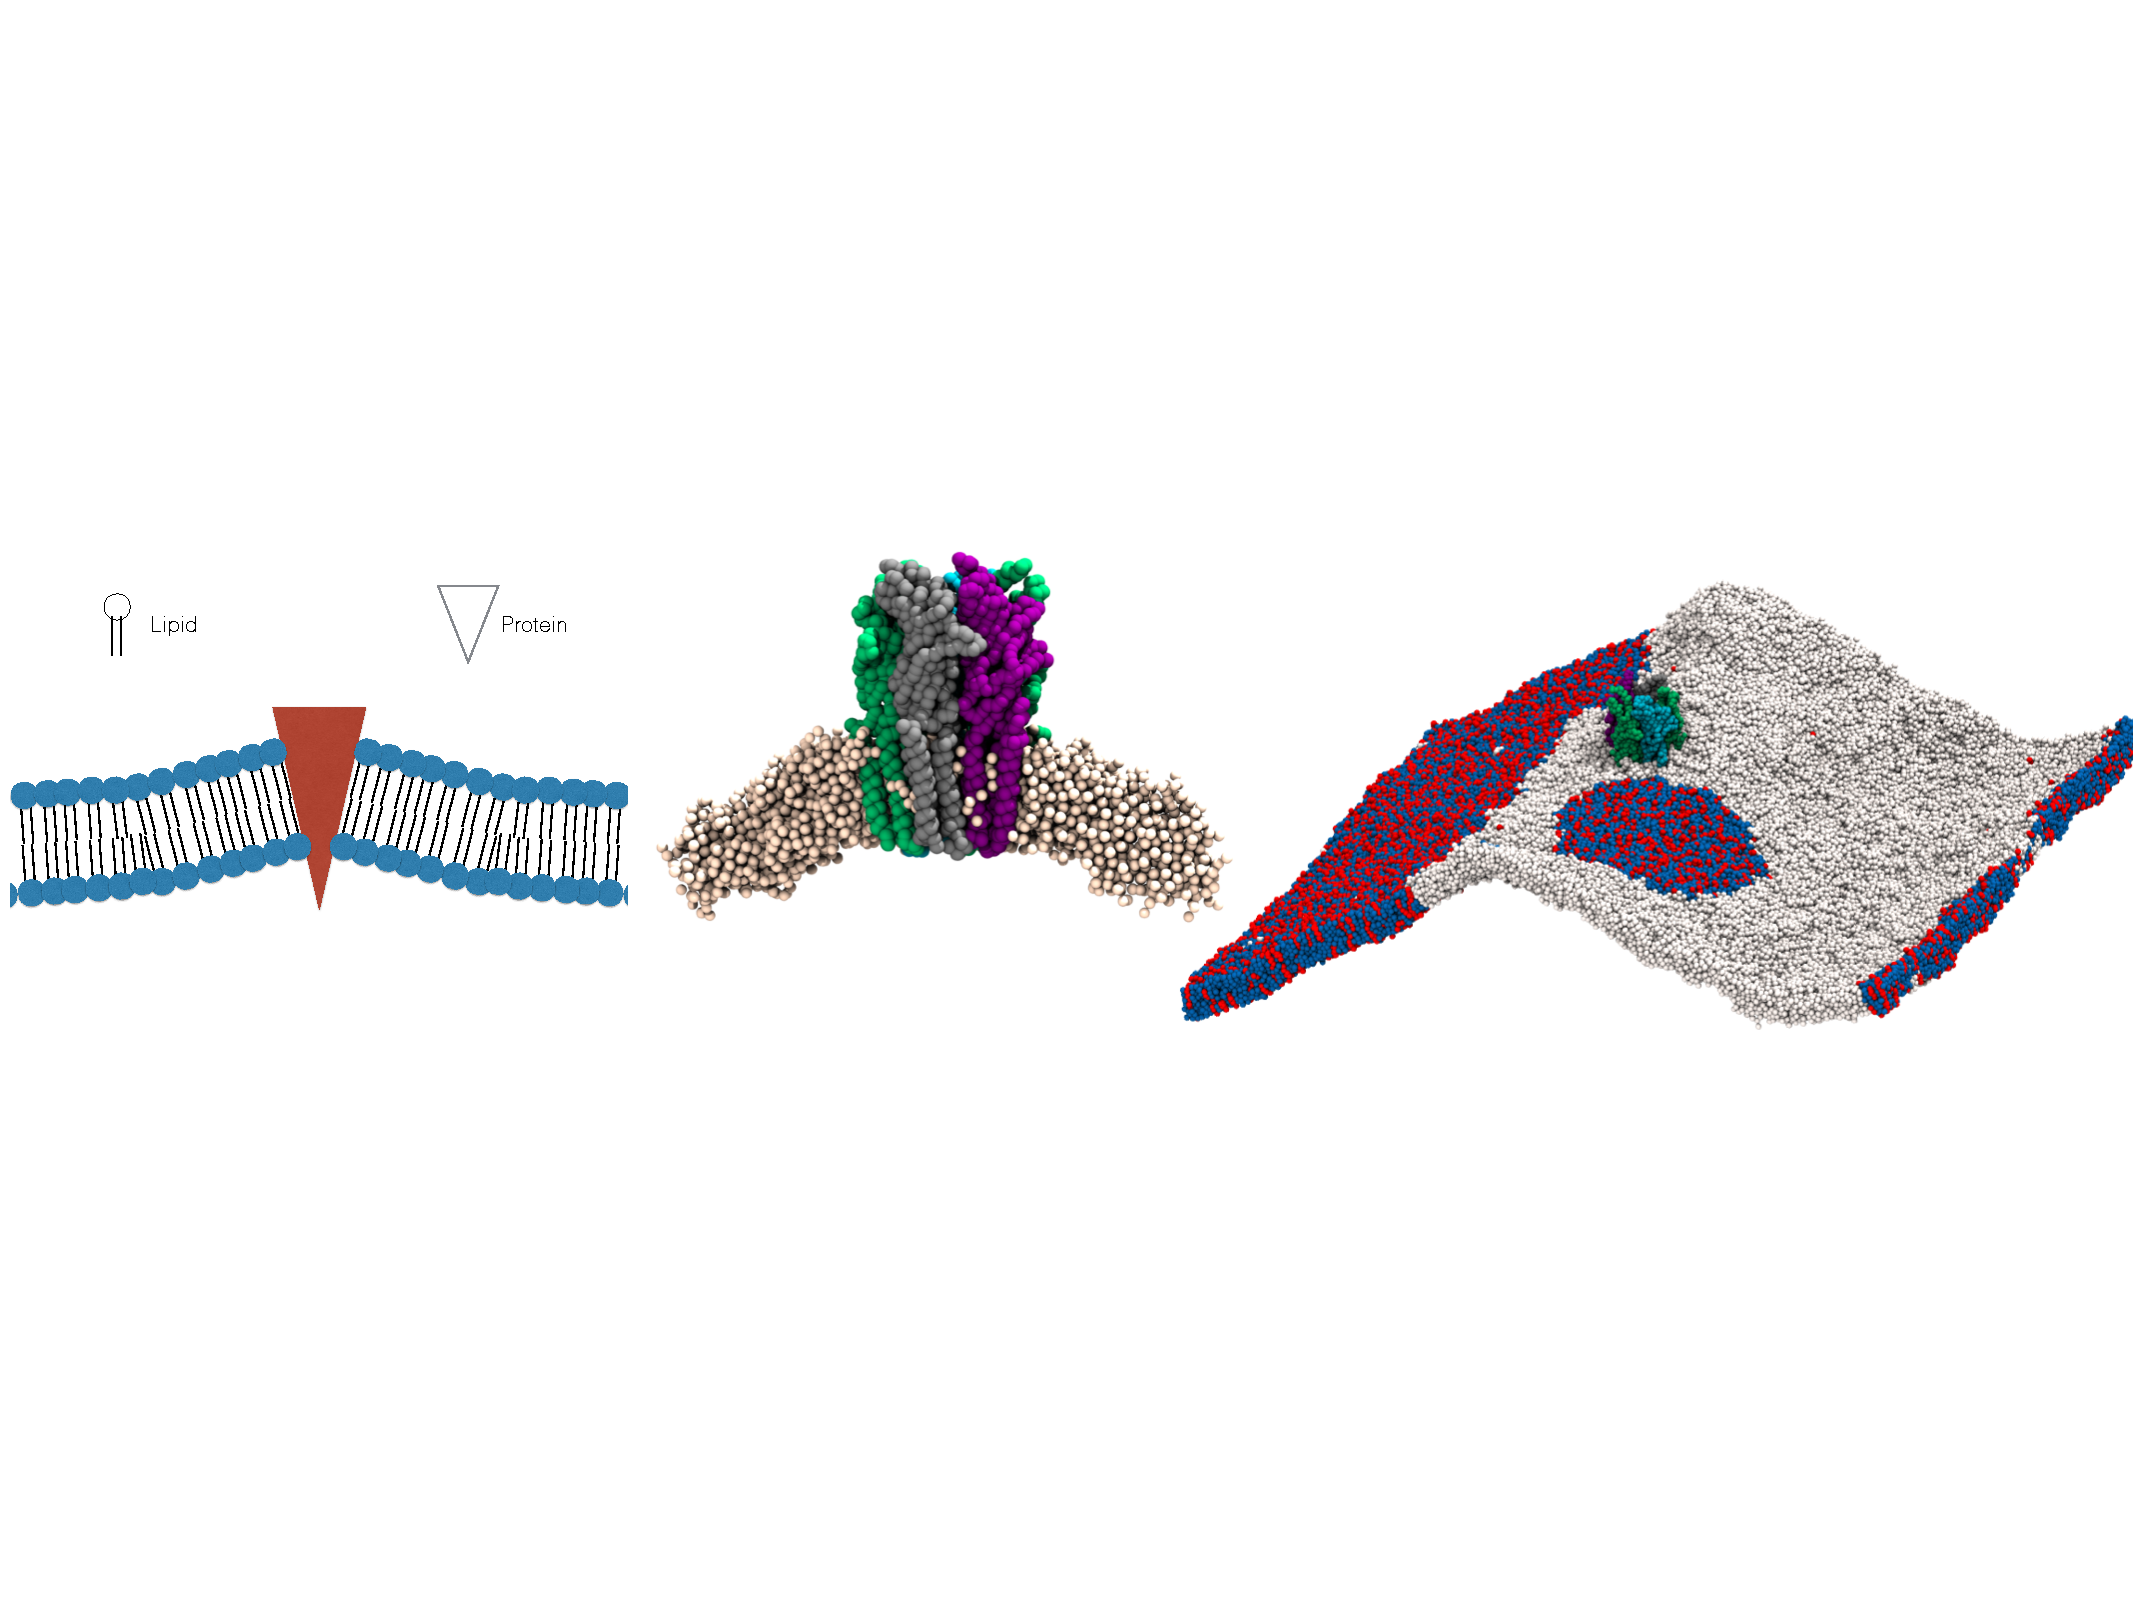
\includegraphics[width=1\linewidth]{./F31/Curvature4.pdf}
	\caption{Possible role of membrane flexibility in determining nAChR partitioning. (A) A schematic representation of predicted membrane deformation around a cone-shaped protein, as described in Goulian et al, \cite{Goulian1996} in which the protein imposes constraints on the slope of the membrane at the interface with the protein (B) Cross-sectional cut of simulation-frame showing membrane deformation around nAChR embedded in an $l_{do}$ phase composed of DHA-PE (white). (C) Phase-boundary partitioning in a larger membrane. nAChR is localized at the interface between the $l_{do}$ phase composed of DHA-PE and the $l_o$ phase composed of DPPC (blue) and cholesterol (red). Provided the membrane is sufficiently large, partitioning at the boundary permits tangential interaction with the cholesterol-rich $l_o$ domain while the flexible $l_{do}$ domain still absorbs the energetic cost of deformation.}
	\label{fig:deform}
\end{figure}

\begin{figure}[t!]
	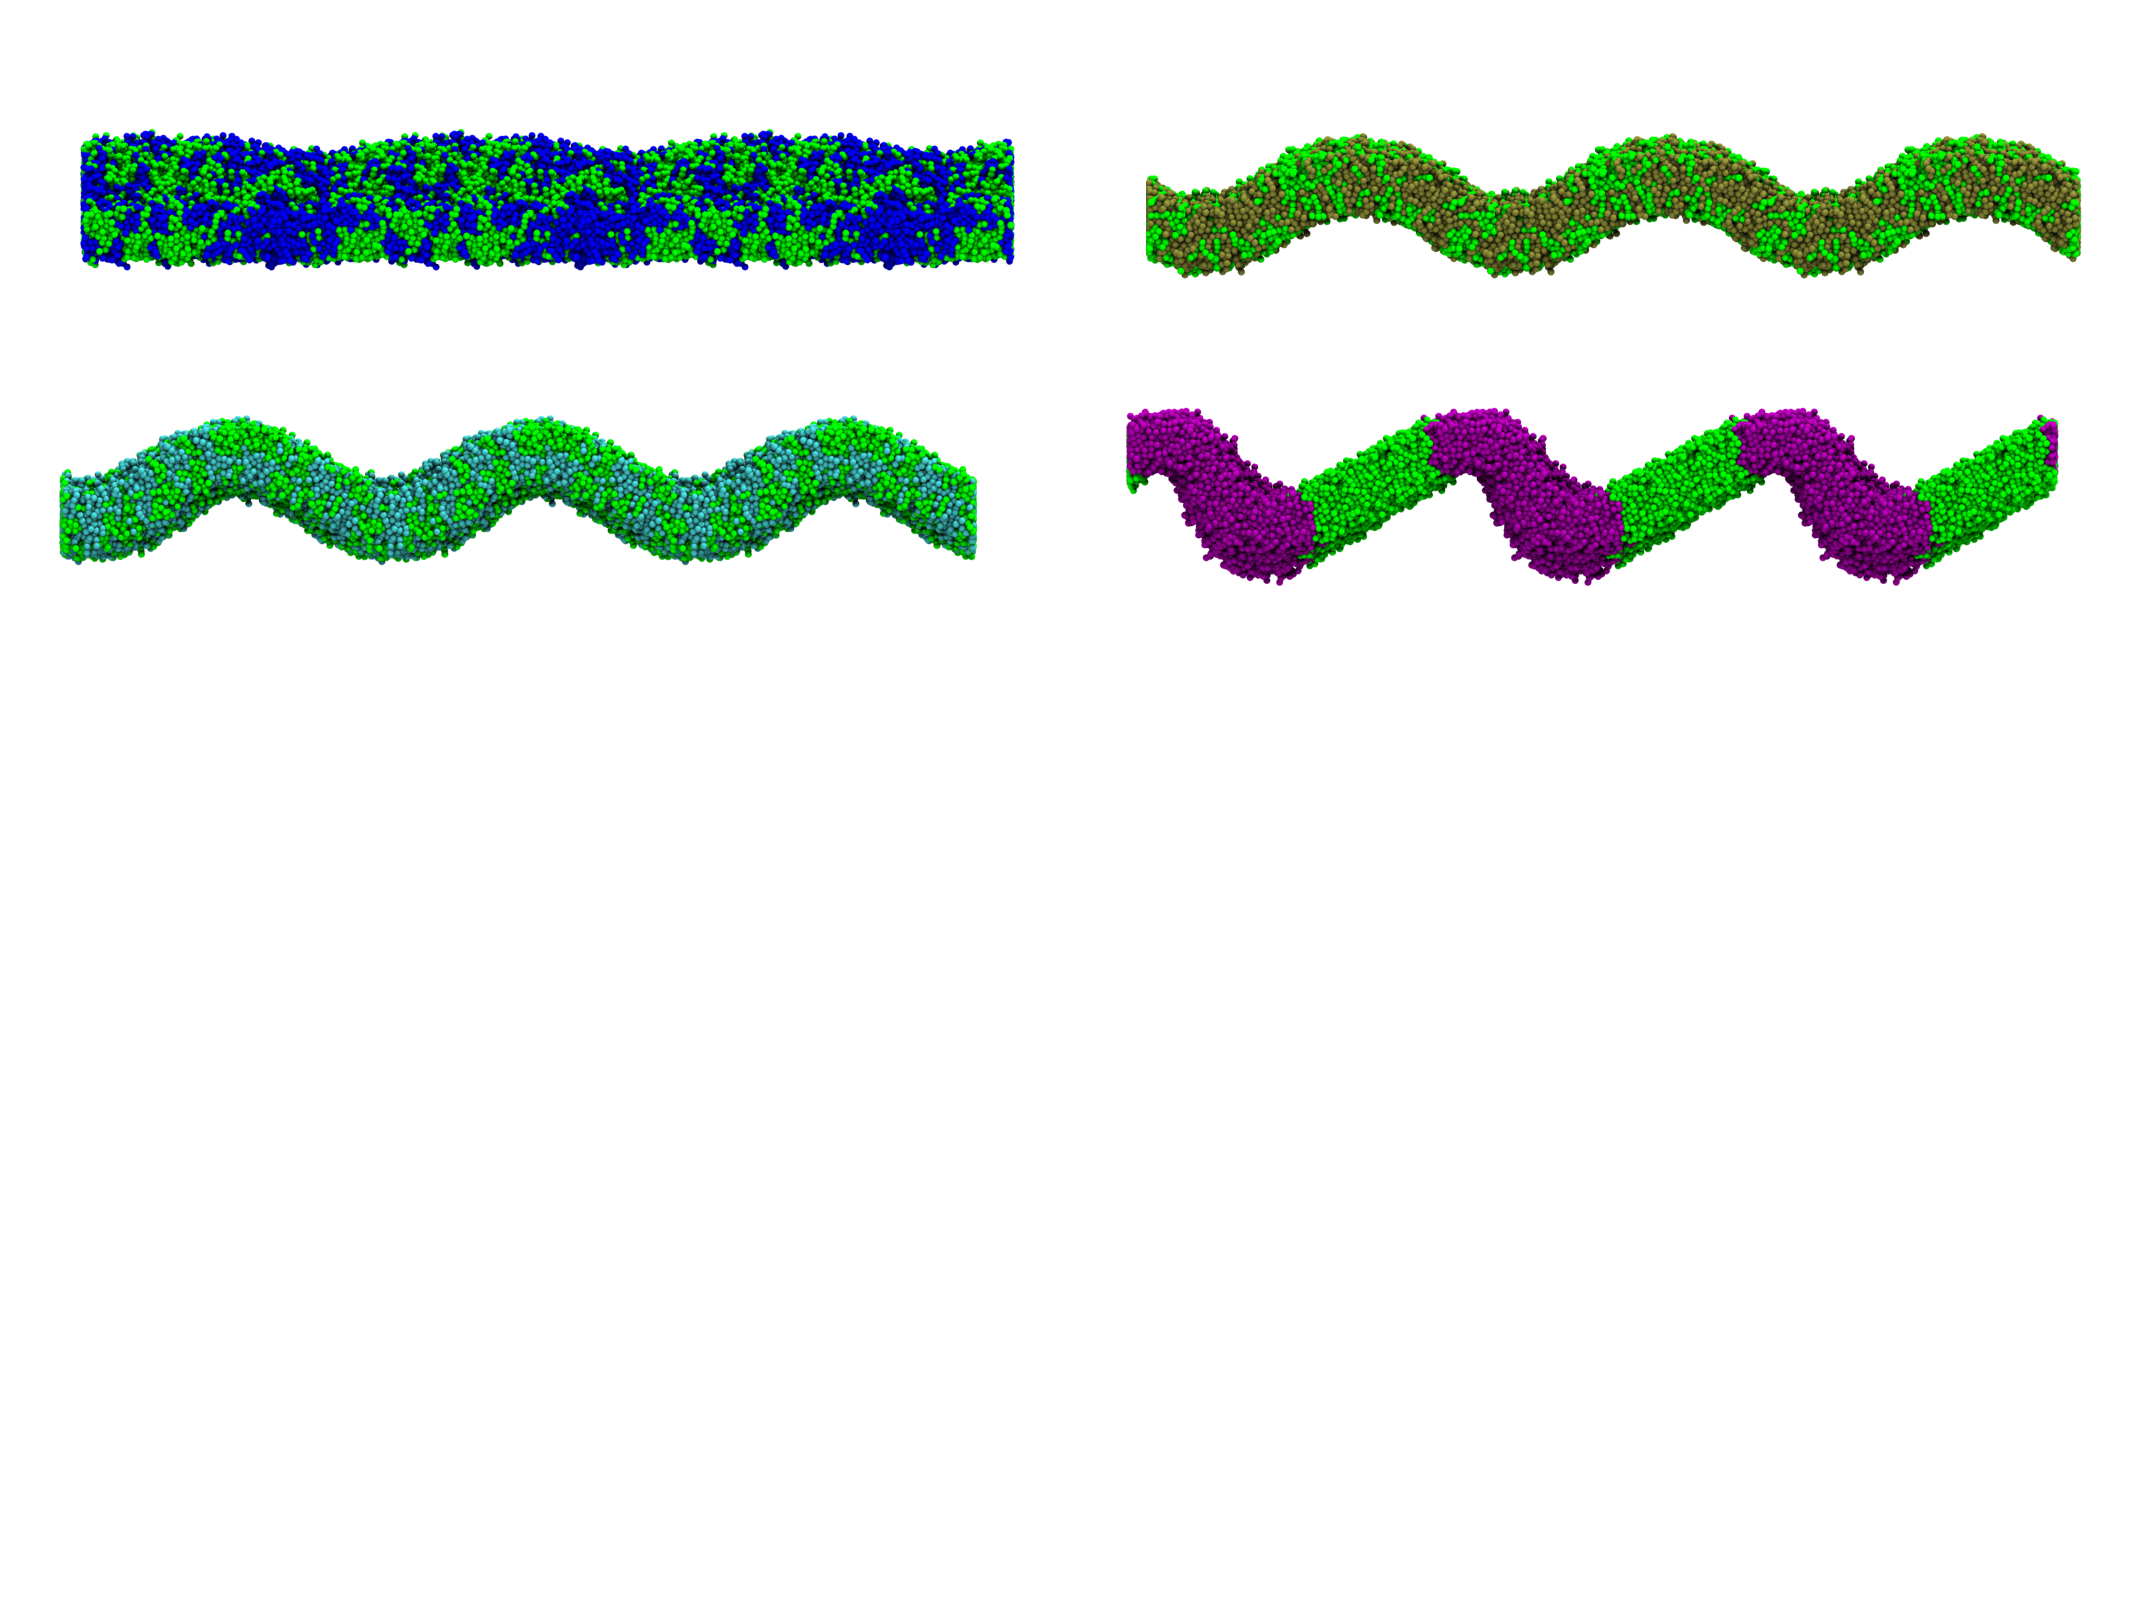
\includegraphics[width=1\linewidth]{./F31/MultiImageElastic.pdf}
	\caption{ Binary, randomly-mixed membranes with increasing thermal undulations and decreasing bending modulus $k_c$. We predict that the more flexible membranes (lower $k_c$) will accommodate a cone shaped protein with reduced energetic costs. The bending modulus $k_c$ can be measured from the thermal undulation spectrum, as well as additional methods appropriate for small membranes. Aim 3 proposes implementation of these methods into a plugin for the widely used analysis-software VMD. For the purpose of this image, saturated lipids are green, while unsaturated lipids are brown, cyan, and purple.}
	\label{fig:elast}
\end{figure}

As one example, neurotransmitter receptors must cluster at high density for efficient neurotransmission, and effects of lipid composition on membrane organization may serve an important modulatory role for an organism's ion channel functionality. The high density of nAChR clusters found in the postsynaptic membrane of the mature neuromuscular junction ($10^4$$\mu m^{-2}$) is well-established to be stabilized by dimerization of nAChRs via binding of the cytoplasmic peripheral membrane protein rapsyn \cite{Zuber_Structure_2013}. This process is also sensitive to membrane composition, particularly cholesterol. It has been frequently hypothesized \cite{Zhu2006,Bruses2001} that initial stages of clustering may require clustering via lipid domains, but experiments investigating whether nAChRs partition into lipid domains have been inconclusive \cite{Bermdez_Partition_2010,Perillo2016}.

Such experiments have focused primarily on detecting partitioning into liquid-ordered ($l_o$ ) domains, which is often detected differently than partitioning into $l_{do}$ domains; in my preliminary simulations we observe partitioning of nAChRs into the $l_{do}$ domain (Figure \ref{fig:ooct}). Partitioning into $l_{do}$ domains would also cluster receptors and be cholesterol dependent, but would be a less effective mechanism in low cholesterol membranes, such as oocytes.

%\subsection{Innovation of Research}

Our observation that nAChR partitions into $l_{do}$ domains was surprising because these domains are very low in cholesterol; the simplest hypothesis to explain cholesterol-sensitivity of nAChR function and oligomerization was that nAChR would partition to the cholesterol rich $l_o$ “raft” phase, although experimental data has been inconclusive.

Direct visualization, using computational microscopy, of the $l_{do}$ domain around nAChR in the MD simulation trajectories revealed a deformation of the membrane around the cone-shape of the TMD (Figure \ref{fig:deform}). This type of deformation was predicted for a general cone shape protein two decades earlier, based on analytical elasticity theories of protein-induced membrane deformations \cite{Goulian1996,Weikl1998} but has not, to our knowledge, been used to predict partitioning preferences of proteins. According to these theories, the energetic penalty for the membrane deformation should increase with the bending rigidity $k_c$, so a significantly more flexible $l_{do}$ phase would be the natural preferred phase for a single receptor.

My approach for this aim is to better determine the role of membrane flexibility in pLGICs partitioning; this has not previously been considered in simulation or experimental design, but it will provide essential insight into whether domain preferences are likely to be more sensitive to pLGIC sequence or to differences in domain rigidity.

%\subsection{Approach of Research}

If partitioning of pLGICs within domain-forming membranes is driven by membrane elasticity and the requirement for a flexible membrane around the cone-shaped protein, partitioning will be strongly sensitive to changes in lipid composition that affect flexibility or spontaneous curvature of $l_o$ and/or $l_{do}$ phases, and only weakly sensitive to pLGIC sequence, since pLGICs are structurally conserved. For example neuromuscular nAChR and GABA(A) receptor$ \alpha 1\beta 3\gamma 2$ $\alpha$ subunit's TMD share $\sim 20 \%$ identity \cite{jalv}, however it is unclear why either partition similarly. If partitioning is instead driven by specific interactions with lipids, it will be far more sensitive to pLGIC sequence, particularly the presence of bulky versus small residues in the TMD. 

My approach will involve first choosing purposeful pLGIC (GABA(A) receptor, glycine receptor, 5HT-3 receptor, and prokaryotic pLGICs such as GLIC or ELIC). Next, using multiple  multiple mutations to nAChR M1, M3, and M4 helices, to sequences of these other pLGICs. Lastly, adjust relative membrane elasticity parameters by e.g. increasing or decreasing membrane asymmetry or increasing or decreasing chain length. The effects of modifications on differences in elastic parameters will be quantified using the approach developed in Aim 3.

%As an example, comparing the sequence of TMDs for $\alpha$ subunits of neuromuscular nAChR and GABA(A) receptor$ \alpha 1\beta 3\gamma 2 $ shows $\sim 20 \% $ identity \cite{jalv}. Potentially suggesting that GABA(A) may not partition into the $l_{do}$. Interestingly the initial ternary DPPC:PUFA:CHOL membranes simulations show GABAAR with similar partitioning as nAChR. GABA(A) is currently running in an oocyte composition as a comparison. 